%%%%%%%%%%%%%%%%%%%%%%%%%%%%%%%%%%%%%%%%%%%%%%%%%%%%%%%%%%%%%%%%%%%%%%%%%%%%%%%%%%%%
% Document data
%%%%%%%%%%%%%%%%%%%%%%%%%%%%%%%%%%%%%%%%%%%%%%%%%%%%%%%%%%%%%%%%%%%%%%%%%%%%%%%%%%%%
\documentclass[12pt]{article} %report allows for chapters
%%%%%%%%%%%%%%%%%%%%%%%%%%%%%%%%%%%%%%%%%%%%%%%%%%%%%%%%%%%%%%%%%%%%%%%%%%%%%%%%%%%%
\usepackage{preamble}

\newcommand{\curvegamma}{\boldsymbol{\vec{\gamma}}}
\newcommand{\tangentgamma}{\boldsymbol{\dot{\vec{\gamma}}}}
\newcommand{\normalgamma}{\boldsymbol{\ddot{\vec{\gamma}}}}
%\newcommand{\forcevec}{\boldsymbol{\vec{F}}}
\newcommand{\rvec}{\boldsymbol{\vec{r}}}
\newcommand{\grad}{\boldsymbol{\vec{\nabla}}}
\usepackage{multicol}

\begin{document}

\begin{center}
   \textsc{\large MATH 272, Worksheet 1, \emph{Solutions}.}\\
   \textsc{Curves, scalar fields, and partial derivatives.}
\end{center}
\vspace{.5cm}

\begin{problem}
    Consider the curve 
    \[
    \curvegamma(t) = \begin{pmatrix} (5+3\cos(8t))\cos(t) \\ (5+3\cos(8t))\sin(t) \\ 3\sin(8t) \end{pmatrix}.
    \]
    \begin{enumerate}[(a)]
        \item Plot this curve from $t=0$ to $t=2\pi$.
        \item Compute the tangent (velocity) vector $\tangentgamma(t)$.
        \item Compute the normal (acceleration) vector $\normalgamma(t)$.
        \item Compute the following 
        \[
        \int_0^{2\pi} \left| \normalgamma(t) \right| dt,
        \]
        which is closely related to the total curvature of the curve.  Indeed, this would be the total force applied to an object of mass $m=1$.
    \end{enumerate}
\end{problem}
\begin{solution}~
\begin{enumerate}[(a)]
    \item Here is a plot of the curve $\curvegamma$. The color green changing to red represents the parameter $t$.
    \begin{figure}[H]
        \centering
        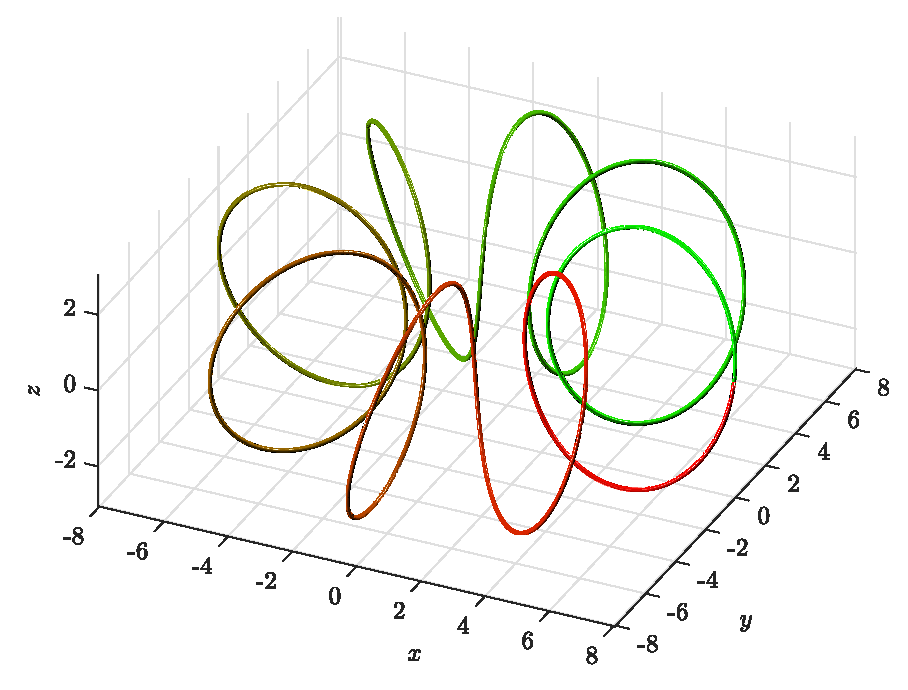
\includegraphics[width=.8\textwidth]{figures/1a}
    \end{figure}

    \item Here we have the components 
    \begin{align*}
    \gamma_1 &= (5+3\cos(8t))\cos(t),\\
    \gamma_2 &= (5+3\cos(8t))\sin(t),\\
    \gamma_3 &= 3\sin(8t).
    \end{align*}
    Taking the $t$ derivatives of these functions yields
    \begin{align*}
    \dot{\gamma_1} &= \sin(t)(-5-3\cos(8t))-24\sin(8t)\cos(t),\\
    \dot{\gamma_2} &= \cos(t)(5+3\cos(8t))-24\sin(8t)\sin(t),\\
    \dot{\gamma_3} &= 24 \cos(8t).
    \end{align*}
   Hence, the tangent vector to $\curvegamma$ at time $t$ is then
    \[
    \tangentgamma(t) = \begin{pmatrix}  \sin(t)(-5-3\cos(8t))-24\sin(8t)\cos(t) \\
                        \cos(t)(5+3\cos(8t))-24\sin(8t)\sin(t) \\
                        24 \cos(8t) \end{pmatrix}.
    \]

    \item Analogously, we find the normal vector. Taking another $t$ derivative of the previous functions yields
    \begin{align*}
    \ddot{\gamma_1} &= 48\sin(8t)\sin(t)-5\cos(t)(39\cos(8t)+1),\\
    \ddot{\gamma_2} &= -48\sin(8t)\cos(t)-5\sin(t)(39\cos(8t)+1),\\
    \ddot{\gamma_3} &= -192 \sin(8t).
    \end{align*}
   Hence, the tangent vector to $\curvegamma$ at time $t$ is then
    \[
    \normalgamma(t) = \begin{pmatrix}  48\sin(8t)\sin(t)-5\cos(t)(39\cos(8t)+1) \\
                        -48\sin(8t)\cos(t)-5\sin(t)(39\cos(8t)+1) \\
                        -192 \sin(8t) \end{pmatrix}.
    \]

    \item Using WolframAlpha to help simplify our expression, we can find
    \[
    \left| \normalgamma(t) \right| = \sqrt{1143\sin^2(8t)+1950\cos(8t)+38050}.
    \]
    Once again, we can use WolframAlpha to integrate and find
    \[
    \int_0^{2\pi} \left| \normalgamma(t) \right| dt \approx 1234.58.
    \]
\end{enumerate}
\end{solution}

\newpage
\begin{problem}~
\begin{enumerate}[(a)]
\item Write an equation for a curve
\[
\curvegamma \colon \R \to \R^3,
\]
satisfying:
\begin{itemize}
    \item Starts with $\curvegamma(0)=\begin{pmatrix} 0 \\ 0 \\ 0 \end{pmatrix}$.
    \item Ignoring the $z$-component, makes a spiral emanating from the origin.
    \item Moves upward at a constant rate in the $z$-direction.
\end{itemize}
Plot this curve that you made to verify that it is correct.
\item Find the tangent vector $\tangentgamma(t)$ to this curve.
\item Find the normal vector $\normalgamma(t)$ to this curve.
\end{enumerate}
\end{problem}
\begin{solution}
\begin{enumerate}[(a)]
    \item If we ignore the $z$-component at first, we can note that choosing $\begin{pmatrix} r\cos(\omega t) \\ r\sin(\omega t) \end{pmatrix}$ gives us a circular curve of radius $r$ in the $xy$-plane. Note that $\omega$ is the angular frequency of rotation in the $xy$-plane. If we allow $r$ to grow from $0$ over time, then we will see a spiral. Perhaps we just choose $\begin{pmatrix} t\cos(t) \\ t\sin(t) \end{pmatrix}$ for the portion of the curve in the $xy$-plane. If we want this curve to move upward in the $z$-direction, then we could choose the third component of our space curve to be, for example, $ct$ for any constant $c$ (there are a multitude of other options as well!). Let us take $c=1$ and $\omega=5$. Putting this together yields the space curve
    \[
    \curvegamma(t) = \begin{pmatrix} t\cos(t) \\ t\sin(t) \\ t \end{pmatrix}.
    \]
    Here is a plot of this curve from $t=0$ to $t=2\pi$ using the same colorscale as in Problem 1.
    \begin{figure}[H]
        \centering
        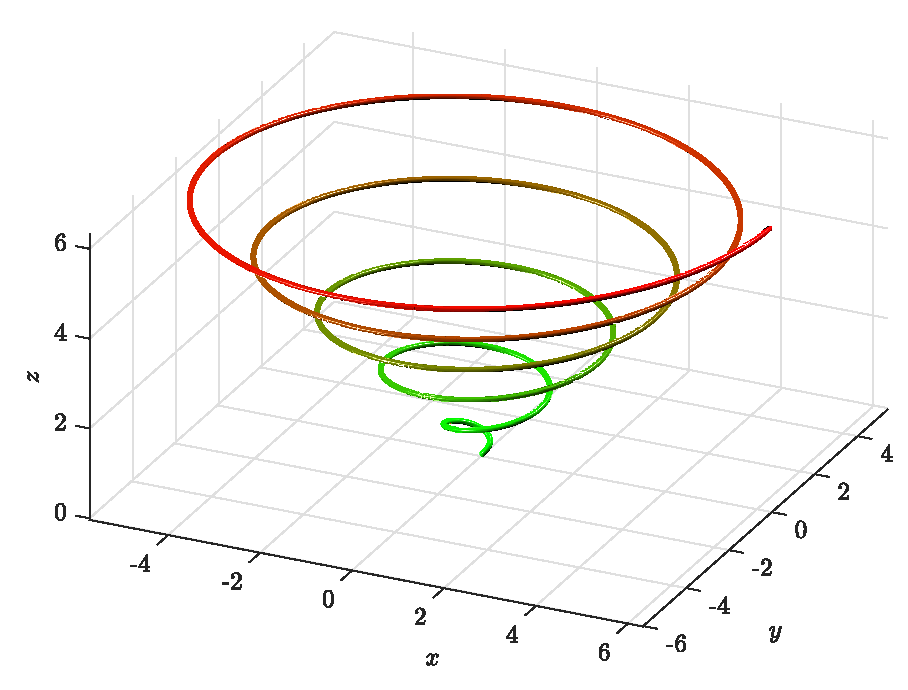
\includegraphics[width=.8\textwidth]{figures/2a}
    \end{figure}

    \item The tangent vector to this curve is
    \[
    \tangentgamma(t) = \begin{pmatrix} \cos(t) - t\sin(t) \\ \sin(t)+t\cos(t) \\ 1 \end{pmatrix}.
    \]
    
    \item Likewise, the normal vector is
    \[
    \normalgamma(t) = \begin{pmatrix} -2\sin(t)-t\cos(t) \\ 2 \cos(t)-t\sin(t) \\ 0 \end{pmatrix}.
    \]
\end{enumerate}
\end{solution}

\newpage
\begin{problem} Consider the two dimensional scalar function 
\[
f(x,y)=e^{\frac{xy}{x^2+y^2-1}}.
\]  
    \begin{enumerate}[(a)]
        \item Plot the graph of this function $(x,y,f(x,y))$ for $x^2+y^2<1$.  
        \item Plot the graph for $x^2+y^2>1$.  
        \item Compute $\frac{\partial f}{\partial x}$ and $\frac{\partial f}{\partial y}$.
        \item Compute all second partial derivatives of $f$.
    \end{enumerate}
\end{problem}
\begin{solution}
\begin{enumerate}[(a)]
    \item Here is a graph of the function for $0<x^2+y^2<0.9$. 
    \begin{figure}[H]
        \centering
        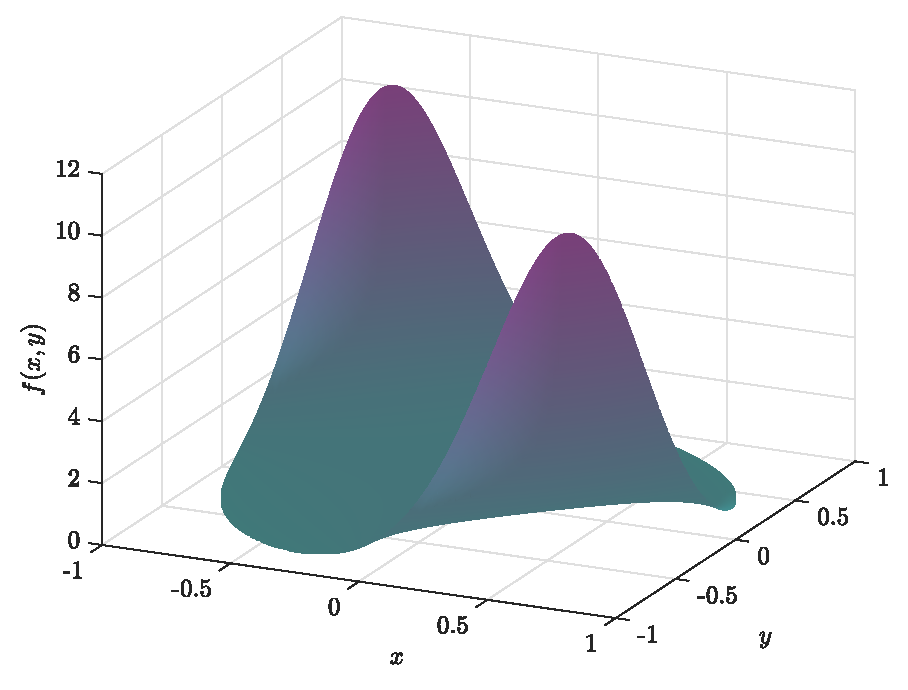
\includegraphics[width=.8\textwidth]{figures/3a}
    \end{figure}

    \item Here is a graph of the function for $x^2+y^2>1.2$. 
    \begin{figure}[H]
        \centering
        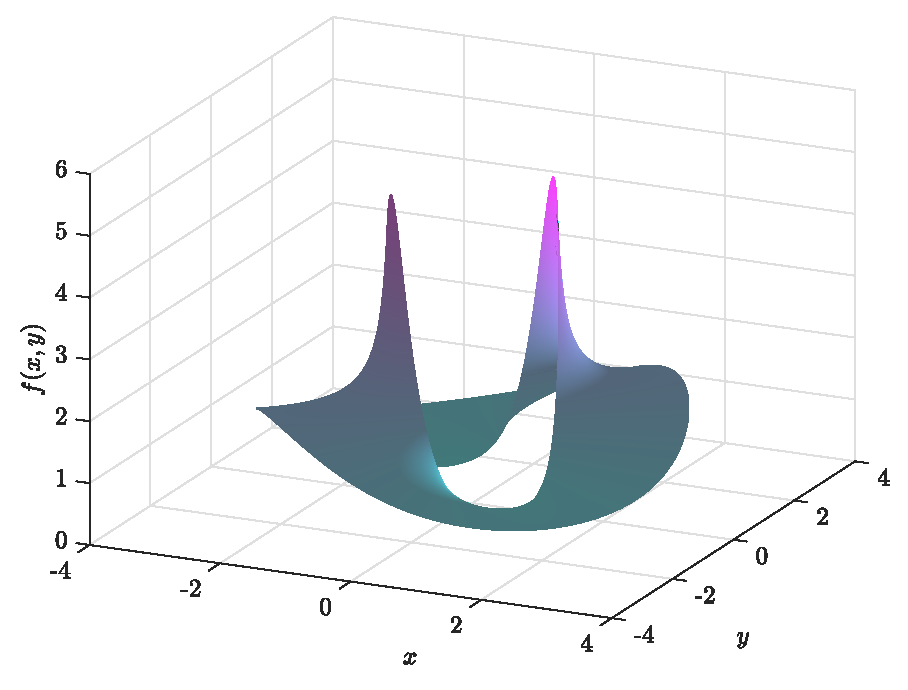
\includegraphics[width=.8\textwidth]{figures/3b}
    \end{figure}

    \item We have
    \begin{align*}
    \frac{\partial f}{\partial x} &= \frac{y(-x^2+y^2-1)}{(x^2+y^2-1)^2}e^{\frac{xy}{x^2+y^2-1}} ,\\
    \frac{\partial f}{\partial y} &= \frac{x(x^2-y^2-1)}{(x^2+y^2-1)^2} e^{\frac{xy}{x^2+y^2-1}}.\\
    \end{align*}

    \item The second partials are then
    \begin{align*}
    \frac{\partial^2 f}{\partial x^2} & = e^{\frac{xy}{x^2+y^2-1}}\left[\left(\frac{y}{x^2+y^2-1}-\frac{2x^2y}{(x^2+y^2-1)^2}\right)^2 +\left( \frac{8x^3y}{(x^2+y^2-1)^3}-\frac{6xy}{(x^2+y^2-1)^2}\right)\right],\\
    \frac{\partial^2 f}{\partial x \partial y}  &= -\frac{e^{\frac{x y}{x^2 + y^2 - 1}}}{(x^2 + y^2 - 1)^4} (x^6 + x^5 y - x^4 (5 y^2 + 1) - 2 x^3 y^3 + x^2 (-5 y^4 + 6 y^2 - 1) \\
        &+ x y (y^4 - 1) + (y^2 - 1)^2 (y^2 + 1)))\\
    \frac{\partial^2 f}{\partial y^2} & = e^{\frac{xy}{x^2+y^2-1}}\left[\left(\frac{x}{x^2+y^2-1}-\frac{2xy^2}{(x^2+y^2-1)^2}\right)^2 +\left( \frac{8xy^3}{(x^2+y^2-1)^3}-\frac{6xy}{(x^2+y^2-1)^2}\right)\right].
    \end{align*}
\end{enumerate}
\end{solution}

\newpage
\begin{problem}~
Write the equation for a scalar function 
    \[
    f\colon \R^2 \to \R,
    \]
    satisfying,
    \begin{itemize}
        \item Has positive $\frac{\partial f}{\partial x}$ everywhere.  
        \item Has negative $\frac{\partial f}{\partial y}$ everywhere.  
    \end{itemize}
    (\emph{Hint: it may help to try adding single variable functions together. That is, let $f(x,y)=u(x)+v(y)$.})
\end{problem}
\begin{solution}
Let us consider a function $f(x,y)=u(x)+v(y)$ for sake of simplicity as this means
\begin{align*}
    \frac{\partial f}{\partial x} &= \frac{du}{dx},\\
    \frac{\partial f}{\partial y} &= \frac{dv}{dy}.
\end{align*}
Hence, we just need to choose $u(x)$ so it has a positive derivative everywhere and $v(y)$ to have a negative derivative. I'll choose $u(x)=x$ and $v(y)=y$.
\end{solution}

\newpage
\begin{problem}
For the following functions, plot the level sets for $c=-1$, $c=0$, and $c=1$. 
\begin{multicols}{2}
\begin{enumerate}[(a)]
    \item For just $c=1$, plot the level set for $E(x,y,z) = \frac{x^2}{25} + \frac{y^2}{16} + \frac{z^2}{9}$.
    \item $f(x,y,z) = xyz$.
    \item $g(x,y,z) = e^x-y^2-z^2$.
    \item $h(x,y,z) = \sin(x)+\cos(y)-\tanh(z)$.
    \item $p(x,y,z) = \sin^2(x)+\sin^2(y)-\frac{1}{2}\sin(z)$.
    \item $q(x,y,z) = x^2+xy+y^2+sin(yz)$.
    \item One of your own choosing.
\end{enumerate}
\end{multicols}
\end{problem}
\begin{solution}~
\begin{enumerate}[(a)]
    \item Here is a plot for $c=1$ for the function $E(x,y,z)$. This surface is called an \emph{ellipsoid}.
    \begin{figure}[H]
    \centering
        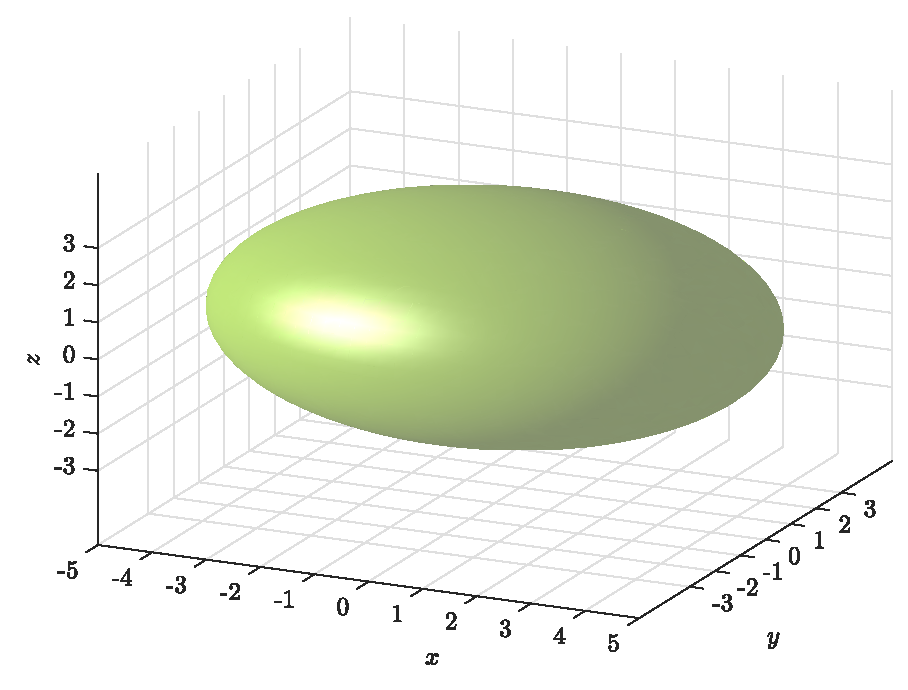
\includegraphics[width=.8\textwidth]{figures/5a}
    \end{figure}

    \item Here is a plots for various values of $c$ for the function $f(x,y,z)$.
    \begin{figure}[H]
    \centering
        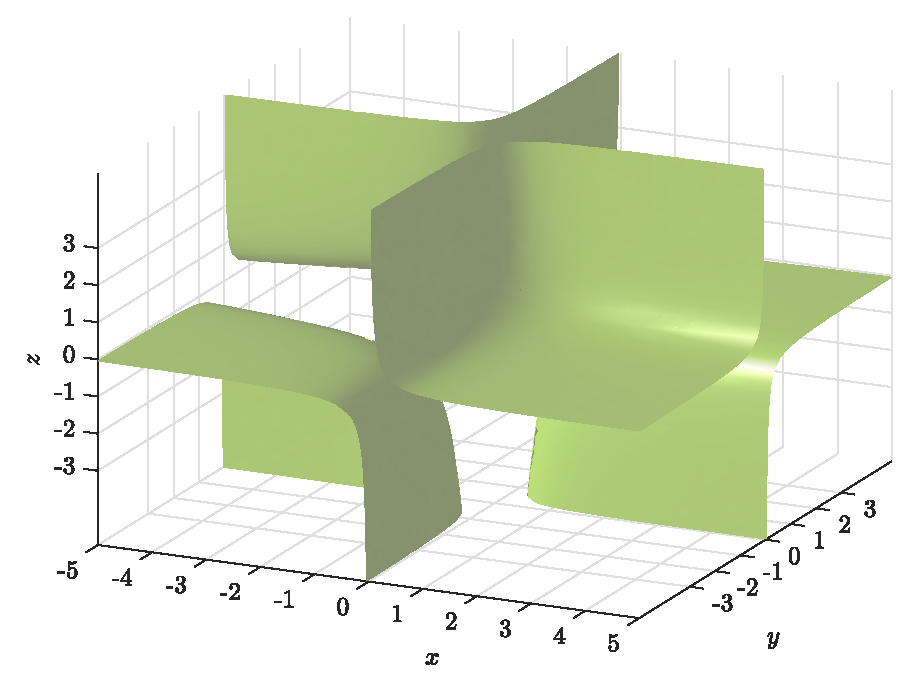
\includegraphics[width=.8\textwidth]{figures/5b_-1}
        \caption{The level set for $f(x,y,z)=-1$.}
    \end{figure}
    \begin{figure}[H]
    \centering
        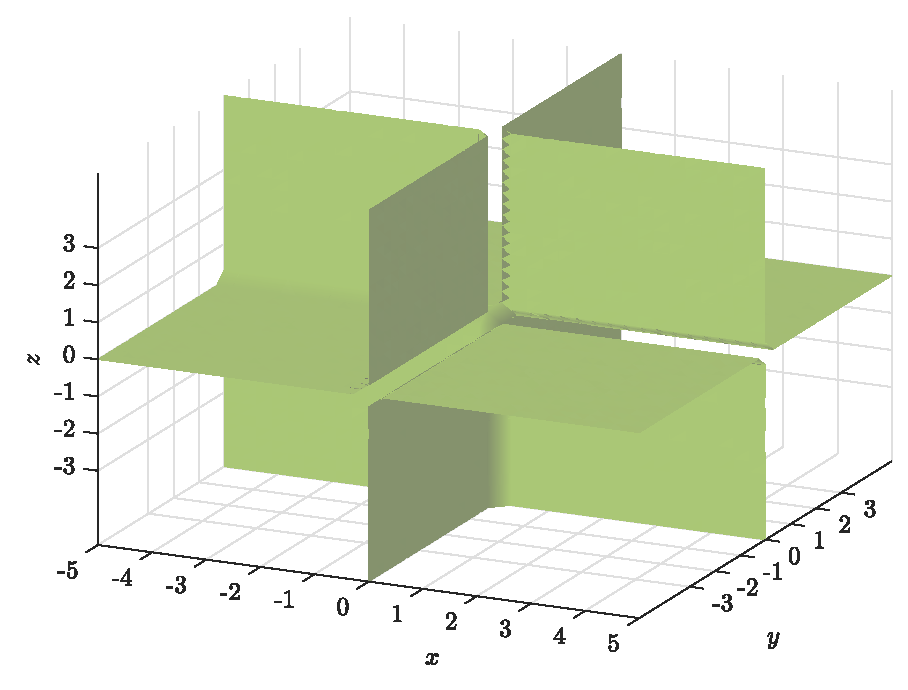
\includegraphics[width=.8\textwidth]{figures/5b_0}
        \caption{The level set for $f(x,y,z)=0$.}
    \end{figure}
    \begin{figure}[H]
    \centering
        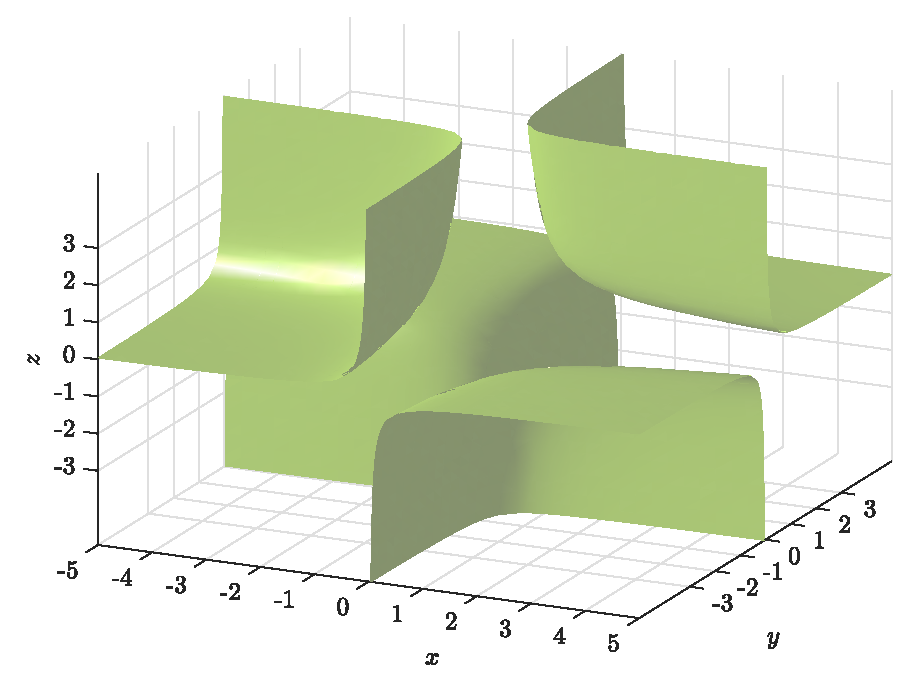
\includegraphics[width=.8\textwidth]{figures/5b_1}
        \caption{The level set for $f(x,y,z)=1$.}
    \end{figure}

\end{enumerate}
\end{solution}






\end{document}
